%!TEX root = ../bachelor.tex
\chapter{Fazit und Ausblick}
\label{ch:summary}

\section{Parallelisierung}

eigentlich quatsch, weil auf raspberry pi

\section{Verbesserung der Linien-Detektion}
Um die Linien-Detektion etwas genauer zu machen, könnte man die Gradientenrichtung des Kantenbilds miteinbeziehen. Dies reduziert die Anzahl falscher Votes und verbessert darüber hinaus die Laufzeit \cite{Gorman1976}. 

probalistic hough?

\section{Verbesserung der Vorwärtsentfaltung}
Das Hauptproblem der Vorwärtsentfaltung sind die Löcher auf dem entfalteten Bild. Um diese schließen zu können, könnte man eine Delaunay-Triangulation durchführen. 
Da das Verfahren jedoch ohne Triangulation schon relativ rechenintensiv ist, und die Rückwärtsentfaltung sehr gute Ergebnisse liefert wurde dieses Möglichkeit nicht weiter untersucht.
Solch eine Triangulation ist beispielhaft in Abbildung \ref{fig:delaunayTriag} abbgebildet. Zum Zwecke der Veranschaulichung wurde hierbei nur ein Teil der Daten benutzt.

\begin{figure}[!htb]
	\centering
	\begin{subfigure}{.9\textwidth}
		\centering
		\includegraphics[angle=-90, width=.8\textwidth]{images/delaunay1.png}
		\caption{Triangulation mit $10\%$ der Punkte}
	\end{subfigure}
	\begin{subfigure}{.9\textwidth}
		\centering
		\includegraphics[angle=-90, width=.8\textwidth]{images/delaunay2.png}
		\caption{Triangulation mit $40\%$ der Punkte}
	\end{subfigure}
	\caption{Delaunay-Triangulation}
	\label{fig:delaunayTriag}
\end{figure}



\section{Verbesserung der Rückwärtsentfaltung}
Aktuell wird die Projektionsmatrix bei der Rückwärtsentfaltung durch \textit{Direct Linear Transformation} bestimmt. Dieses Verfahren minimiert jedoch nicht den Reprojektionsfehler. Besser wäre hier deshalb ein iteratives Verfahren, wie der Levenberg–Marquardt-Algorithmus (konkret für Projektionsmatrizen beschrieben in \cite{Hartley2000}). %wurde beschrieben in hartley und zisserman 
Im Gegensatz dazu könnte auch ein RANSAC-Ansatz verwendet werden. Statt eine optimale Lösung für alle detektierte Samples zu bestimmen, berechnet man wiederholt für sechs Punkte\footnote{sechs Punkte sind mindestens notwendig um eine Projektionsmatrix bestimmen zu können, da es elf unbekannte gibt (siehe Kapitel \ref{s:calib}).} eine Projektionsmatrix und untersucht dann den Reprojektionsfehler für alle anderen Punkte und wählt schließlich die Projektionsmatrix mit dem größten Consensus Set aus. 



%\section{andere Ansätze}\todo{wie am besten einbetten?}
%\textit{Analytical Deformable Templates} ist ein Verfahren zur Detektion von analytischen Kurve, wie beispielsweise einer Ellipse, mittels Optimierung einer Energiefunktion. 
%
%Wir betrachten dazu folgende Funktion, deren Nullstellen wie in Kapitel \ref{s:ellipse}, eine um $\theta$ gedrehte Ellipse, mit Zentrum $(x_0,y_0)$ und Haupt- und Nebenachse $a$ und $b$ beschreiben. 
%\begin{equation*}
%	G(x,y) = \frac{((x - x_0)\cos\theta + (y - y_0)\sin\theta)^2}{a^2} + \frac{((x - x_0)\sin\theta - (y - y_0)\cos\theta)^2}{b^2} - 1
%\end{equation*}
%
%Wir konstruieren eine Energiefunktion:
%\begin{equation*}
%	E = E_M + E_A + E_S,
%\end{equation*}
%die sich zusammensetzt aus einem Term $E_M$, der die Kantenstärke auf dem Ellipsenrand maximiert, sowie einem Term $E_A$ der die Winkelähnlichkeit zwischen Ellipsennormale und Gradientenrichtung maximiert. Darüber hinaus fügen wir einen Term $E_S$ hinzu, der die Ellipse schrumpfen lässt. 
%
%Genauer sehen die Terme wie folgt aus
%\begin{equation*}
%\begin{aligned}
%E_M &= -\alpha\frac{1}{n}\sum_{i=0}^{n-1}I_M(p_i) \\
%E_A &= \beta\frac{1}{n}\sum_{i=0}^{n-1}\left(I_O(pi) - \atant{\left(\frac{\partial G}{\partial y}(p_i), \frac{\partial G}{\partial x}(p_i)\right)}\right)^2 \\
%E_S &= \gamma\frac{1}{n}\sum_{i=0}^{n-2}\abs{p_i - p_{i+1}},
%\end{aligned}
%\end{equation*}
%
%wobei $n$ die Anzahl der Punkte auf dem Ellipsenrand sind. $p_i$ ist definiert als der $i$-te Punkt auf der Ellipse (siehe parametrische Darstellung einer Ellipse).
%Man wählt dabei als Startwert eine Ellipse, deren Zentrum dem Bildzentrum entspricht und deren Hauptachse und Nebenachse möglichst größ sind und bestimmt dann numerisch, beispielsweise durch Gradient Descent, ein Minimum der Funktion. Der Term $E_M$ wird minimal, wenn entlang der Ellipse die Kantenstärke (\textit{\textbf{M}agnitude}) groß ist. Der Term $E_A$ wird minimal wenn die Winkel der Normalenvektoren ähnlich zu denen der Kanten sind (\textit{\textbf{A}ngle}) und $E_S$ wird minimal, wenn die Distanz aufeinanderfolgender Ellipsepunkte klein wird, also die Ellipse als ganzes klein wird (\textit{\textbf{S}ize}). Der Term lässt die Ellipse also schrumpfen. $\alpha, \beta$ und $\gamma$ steuern hierbei den Einluss der einzelnen Terme. Das Minimum der Funktion sollte die äußerste Ellipse im Kalibirierungsmuster sein. Anschließend wird diese Ellipse vom Bild entfernt und man sucht wiederholt Minima der Funktion bis alle Ellipse detektiert wurden. 
%
%Das Problem bei diesem Ansatz, ist dass die Funktion, auch nach starker Gaussglättung, schnell in kleine lokale Minima läuft, obwohl ein wesentlicher stärkeres Minimum in näherer Umgebung wäre. Darüber hinaus muss für ein robustes Optimierungsverfahren der Gradient und im besten Fall sogar die Hesse-Matrix zur Verfügung gestellt werden. 
%
%In Abbildung \ref{fig:deformable} sieht man beispielhaft einen Auschnitt der Energiefunktion, wobei in diesem Fall zwecks Veranschaulichung nur die Haupt- und Nebenachse der Ellipse variable sind. Das Zentrum bleibt das Zentrum des Bildes und der Winkel $\theta$ ist konstant null. Trotz dieser Einschränkungen lässt sich gut erkennen, dass circa bei $a = b = 300$ ein starkes Minimum liegt. Es gibt jedoch neben diesem Minimum in näherer Umgebung kleine irrelevante Minima, wie beispielsweise in $(360, 260)$. Solche "`Becken"' erschweren die Suche nach der nächsten Ellipse erheblich.
%
%
%\begin{figure}[!htb]
%	\centering
%	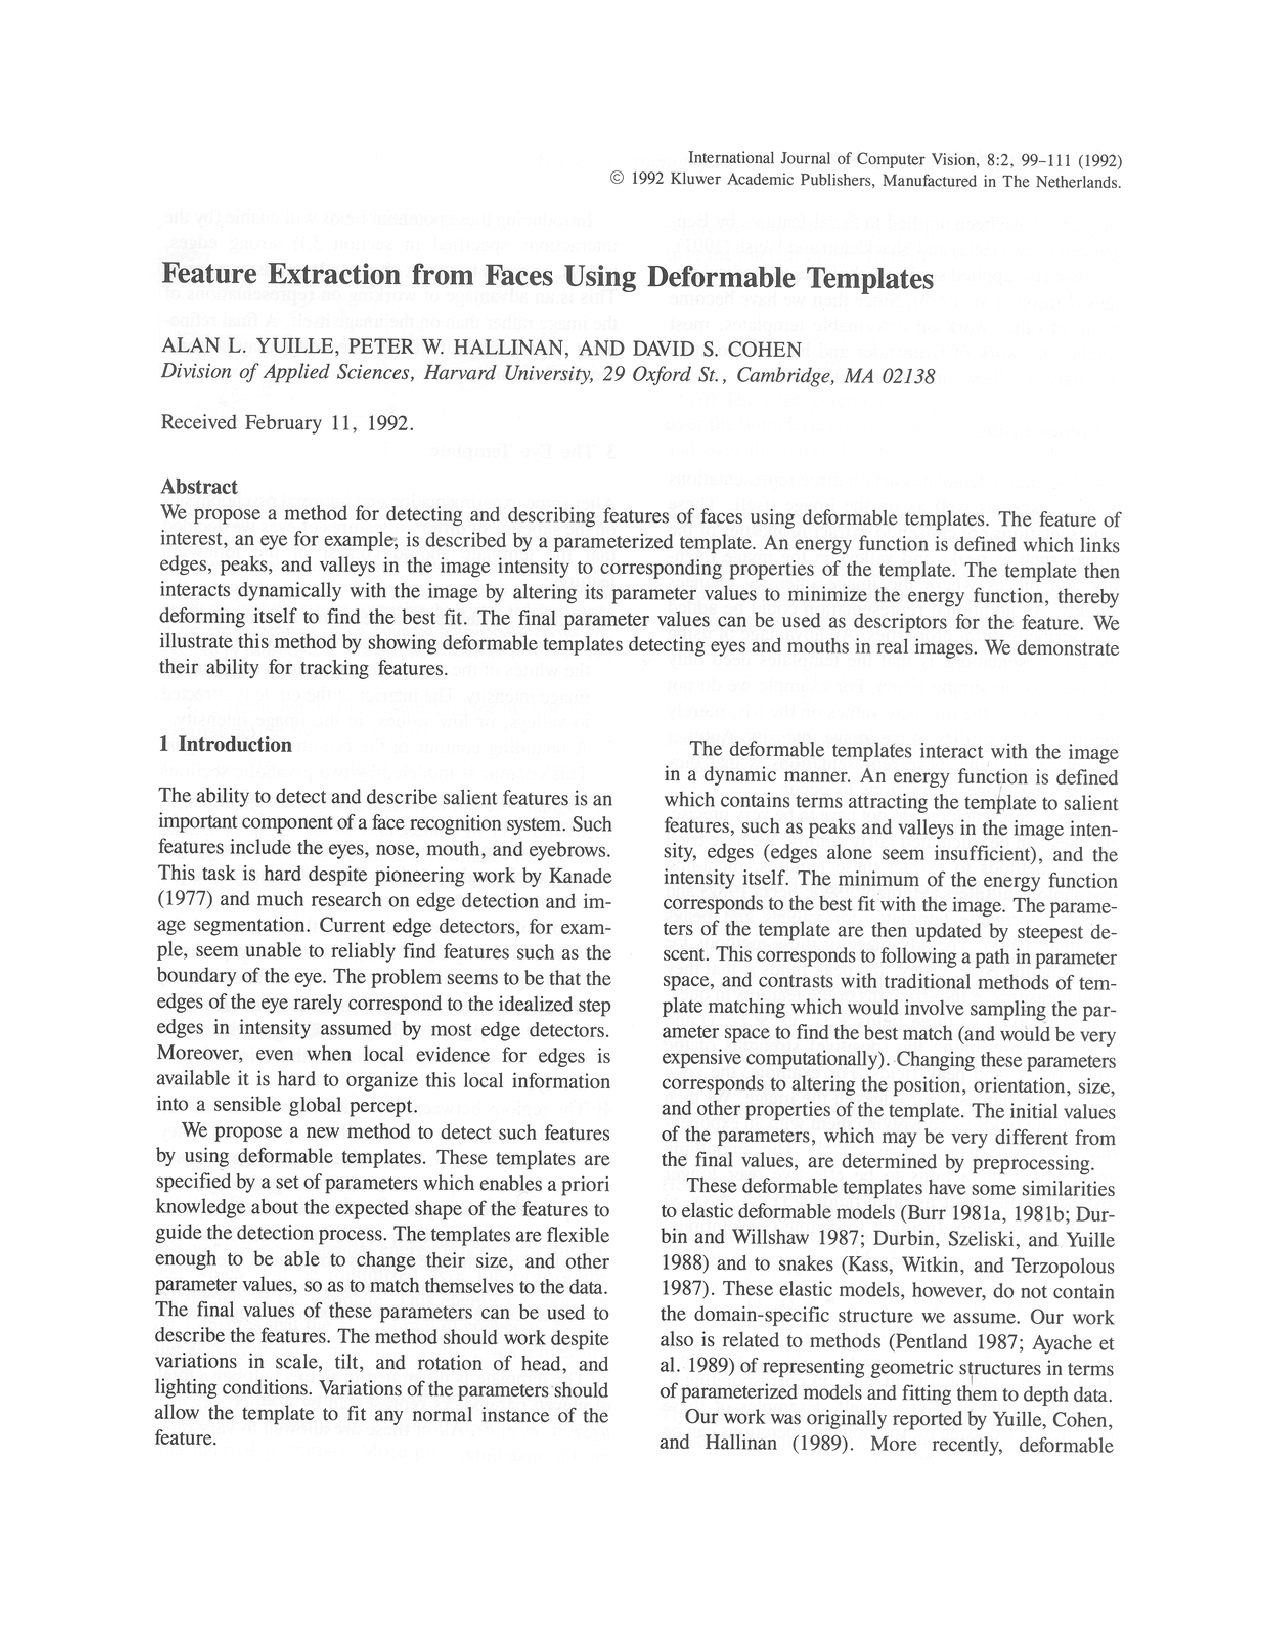
\includegraphics[scale=.4]{images/deformable.png}
%	\caption{Deformable Templates: Ausschnitt der Energiefunktion für variable Haupt- und Nebenachse}
%	\label{fig:deformable}
%\end{figure}




\todo{Literatur überprüfen, insbesondere Seitenangaben}









